\documentclass[a4paper, 10pt, final]{article}
\usepackage{michael}

%% \def\mytitle{Signal and Image Processing 2010}
%% \def\mysubtitle{Handin of mandatory excercise 1}
%% \def\myauthor{Ulrik Bonde}
%% \def\mymail{\mailto{bonde@diku.dk}}
%% \def\mydate{\today}

\title{Signal and Image Processing 2010 \\ Mandatory hand-in exercise 1}
\author{Michael Andersen}
\date{\today}

%% \title{\mytitle}
%% \subtitle{\mysubtitle}

%% \author{\myauthor{} - \mymail}
%% \date{\mydate}

\hypersetup{
colorlinks,%
citecolor=black,%
filecolor=black,%
linkcolor=black,%
urlcolor=black,%
bookmarksopen=false,
pdftitle={Signal and Image Processing 2010 - Mandatory exercise 1},
pdfauthor={Michael Andersen}
}

\begin{document}
\maketitle

\subsection*{Question 1.1}
We are to prove that Fourier transform of a real and even function is real and even.

\begin{equation*}
    \hat{g}(k) = \int_{-\infty}^{\infty}{g(x)\exp(-2\pi ikx)dx}
\end{equation*}
The above equation describes the 1-D Fourier Transformation, the equation is the same as eqn. 2.18 found on page 44 in the Digital Image Processing book.

The above equation can be split into two, and by changing the limits of the integral we change the sign. Lastly we substitute $x = -x$, thereby changing the sign in front of the second integral again.
\begin{align*}
    \hat{g}(k) & = \int_{-\infty}^{0}{g(x)\exp(-2\pi ikx)dx} + \int_{0}^{\infty}{g(x)\exp(-2\pi ikx)dx}\\
               & = \int_{0}^{\infty}{g(x)\exp(-2\pi ikx)dx} - \int_{0}^{-\infty}{g(x)\exp(-2\pi ikx)dx}\\
               & = \int_{0}^{\infty}{g(x)\exp(-2\pi ikx)dx} + \int_{0}^{\infty}{g(-x)\exp(2\pi ikx)dx}
\end{align*}

We now use the fact that we know that $g(x) = g(-x)$ because $g(x)$ is even, this results in the following equation:
\begin{equation*}
  = \int_{0}^{\infty}{g(x)\exp(-2\pi ikx)dx} + \int_{0}^{\infty}{g(x)\exp(2\pi ikx)dx}
\end{equation*}

By applying \textit{Euler's identities} $\cos(\theta) =
\frac{e^{i\theta} + e^{-i\theta}}{2}$. Setting $\theta = 2\pi kx$ and multiplying by $2$. We get the following:

\begin{align*}
  & = 2 \int_{0}^{\infty} {g(x) \frac{e^{i2\pi kx} + e^{-i2\pi kx}}{2}dx} \\
  & = 2 \int_{0}^{\infty}{g(x) \cos{(2\pi kx)}}
\end{align*}

The result $2 \int_{0}^{\infty}{g(x) \cos{(2\pi kx)}}$ only contains real parts, and therefore the result is real. We know that $g(x)$ is even, and the same applies to $\cos{(x)}$. This proves that the Fourier transform of a real and even function is also real and even.

\subsection*{Question 1.2}
We are to find the Fourier tranform of $\delta_{x,x_{0}} + \delta_{x,-x_{0}}$. This is done as follows (calculation has been split into two integrals for ease)first part:
\begin{equation*}
   \int_{-\infty}^{\infty} {\delta_{x,x_{0}} e^{-2\pi ikx}dx}
\end{equation*}
\[
  = e^{-2 \pi ikx_{0}}
\]
This is because of the properties of the $\delta$-function which is only ``active'' when $x = x_{0}$. The other integral is almost symmetrical to the above, being:
\begin{equation*}
   \int_{-\infty}^{\infty} {\delta_{x,-x_{0}} e^{-2\pi ikx}dx}
\end{equation*}
\[
  = e^{2 \pi ikx_{0}}
\]
The combination of the above two equations are:
\[
e^{-2\pi ikx_{0}} + e^{2\pi ikx_{0}}
\]
Again we can apply \textit{Euler's identities}, as we are missing the denominator, we need to multiply the result by $2$
\[
= 2 \cos{(2\pi kx_{0})}
\]

We now need to show the Fourier transform of $\cos{(2\pi
  xu_{0})}$. Trying to integration of this would probably end
horribly. Instead perform a guess based on the above calculation, our
guess being $\frac{1}{2}(\delta_{x,u_{0}} +
\delta_{x,-u_{0}})$. Performing similar steps as above we get:
\begin{align*}
  \hat{g}(k) & = \frac{1}{2} \int_{-\infty}^{\infty} {(\delta_{x,u_{0}} +\delta_{x,-u_{0}})\exp{-2\pi ikx}dx}\\
  & = \frac{1}{2} 2 \cos{(2\pi ku_{0})} \\
  & = \cos{(2\pi ku_{0})}
\end{align*}
Therefore our guess was correct and the result is
$\frac{1}{2}(\delta_{x,u_{0}} + \delta_{x,-u_{0}})$

\subsection*{Question 1.3}
It all depends on the value $\lambda$, as the wave length goes towards $\infty$ the $|k|$ goes towards zero. Therefore as the bass has large wavelength this results in a small value of $|k|$. And vice versa for treble.

\subsection*{Question 1.4}
\subsubsection*{Gray color reduction}
We are to write program that reads in an image and performs a reduction of the number of grayscale colors used in the image and modify/write another that is able to perform resolution reduction.

\begin{figure}[!h]
\centering
\subfloat[]{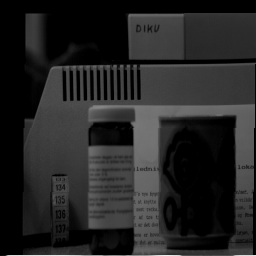
\includegraphics[width=0.3\textwidth]{images/img00}}
\subfloat[]{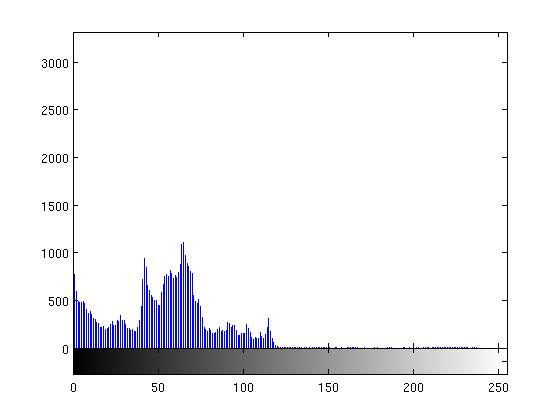
\includegraphics[width=0.45\textwidth]{images/img00h}}
\caption{Original image and histogram, unadjusted}
\label{fig:original}
\end{figure}
The figure \ref{fig:original} shows the original image and its histogram. It can be seen from the histogram that the image does not facilitate the entire gray colormap. Therefore I perform a image adjusting using the built-in \emph{imadjust} in MatLab to convert the picture to use the entire gray colormap, resulting in the image and histogram shown in figure \ref{fig:original_adjusted}. I will be working on the adjusted image for the remaining of this exercise. 

\begin{figure}[!h]
\centering
\subfloat[]{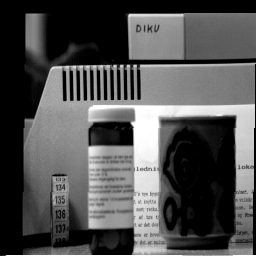
\includegraphics[width=0.3\textwidth]{images/img01}}
\subfloat[]{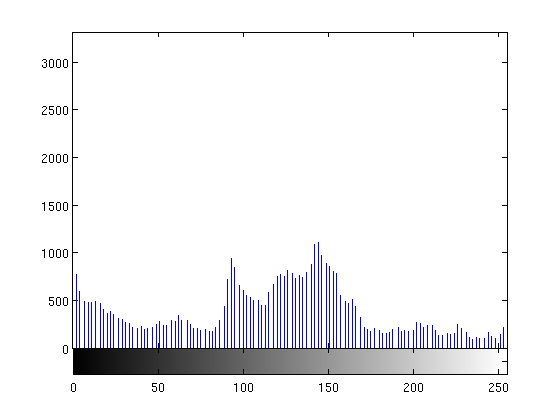
\includegraphics[width=0.45\textwidth]{images/img02}}
\caption{Original image and histogram, adjusted}
\label{fig:original_adjusted}
\end{figure}

It is worth mentioning that without the adjustment of the images
colormap some troubles can arise when reducing the number of grayscale
colors. This is because the algorithm for reducing the colors rely on
the bins generated the built-in MatLab function
\emph{imhist}. Therefore, if the image colormap does not span the
entire colormap some of these bins will be empty, resulting in fewer
colors than expected.

\begin{figure}[!h]
\centering
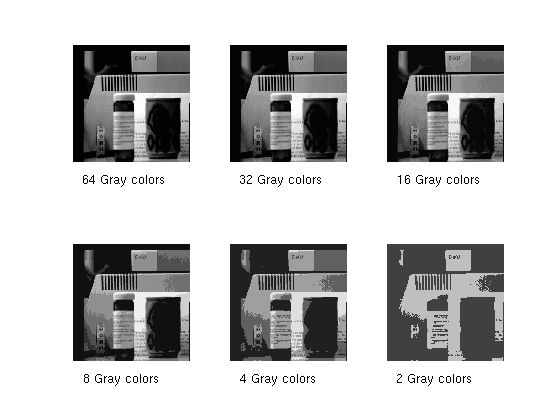
\includegraphics[width=1.0\textwidth]{images/img_reduce_range}
\caption{Reduction range from 64--2 gray colors, adjusted}
\label{fig:reduceGray_range}
\end{figure}
The figure \ref{fig:reduceGray_range} show color reduction from 64--2 in steps of power of 2, meaning $64, 32, \ldots, 2$. Most of the text is still readable with 64 colors (see figure \ref{fig:reduceGray64}), except on the prescription bottle. Seing the picture from a little distance makes it almost impossible to recognize from the original adjusted picture.

\begin{figure}[!h]
\centering
\subfloat[]{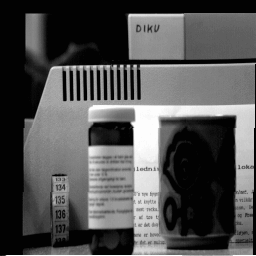
\includegraphics[width=0.3\textwidth]{images/r64}}
\subfloat[]{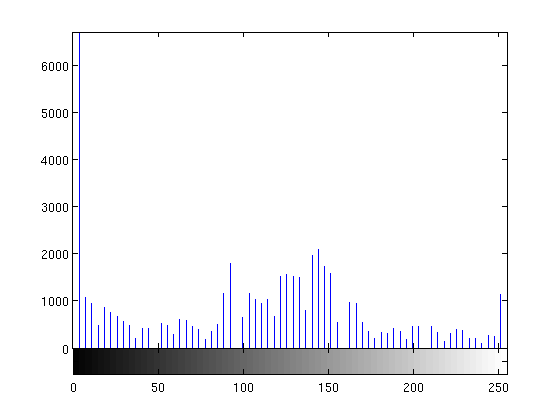
\includegraphics[width=0.45\textwidth]{images/r64h}}
\caption{Reduced to 64 gray colors, image and histogram}
\label{fig:reduceGray64}
\end{figure}

As the color bins are combined, the average of their values are used
to define the new color fill for the previous two colors. When the
colors are reduced to 8 gray colors \ref{fig:reduceGray8} the pattern on
the cup has nearly disappeared. This is a result of the bins
containing the different colors in the pattern has been collapsed into
two colors. The text spelling 'DIKU' is still visible along with the
text on the measuring tape and some of the heading on the paper behind
the prescription bottle and cup.

\begin{figure}[!h]
\centering
\subfloat[]{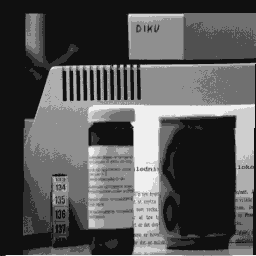
\includegraphics[width=0.3\textwidth]{images/r08}}
\subfloat[]{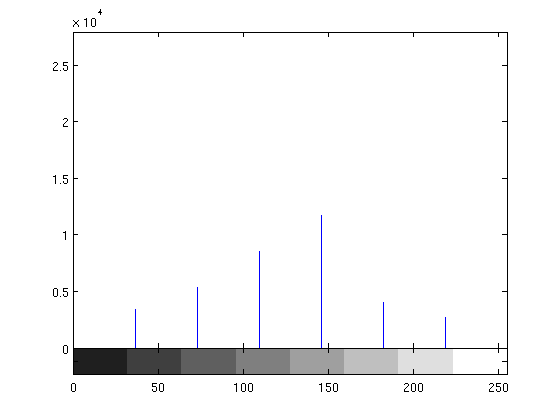
\includegraphics[width=0.45\textwidth]{images/r08h}}
\caption{Reduced to 8 gray colors, image and histogram}
\label{fig:reduceGray8}
\end{figure}

Futher reduction to four colors in figure \ref{fig:reduceGray4}
results in the patter on the cup disappearing. The text on the
prescription bottle is now reduced to gray patches. And only
a few of the numbers on the measuring tape is still visible, depending
on the original light setting. The text 'DIKU' is still visible, this
is a result of the sharp contrast between the text color and the
bright background. Additionally the top of the prescription bottle now
has the same color as the paper behind it, except for the right side
of it, which was dark due to shadows in the original image.

\begin{figure}[!h]
\centering
\subfloat[]{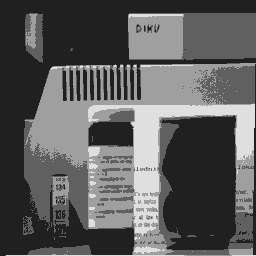
\includegraphics[width=0.3\textwidth]{images/r04}}
\subfloat[]{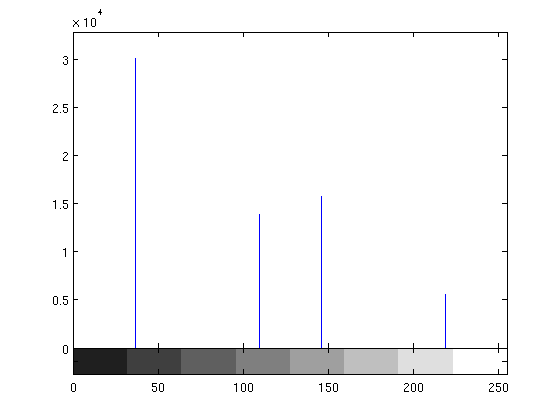
\includegraphics[width=0.45\textwidth]{images/r04h}}
\caption{Reduced to 4 gray colors, image and histogram}
\label{fig:reduceGray4}
\end{figure}

The reduction to two colors makes the image into a binary image
composited of two gray colors with index values around 74 and 192 (see
figure \ref{fig:reduceGray2}). Only the text 'DIKU' is still visible,
the rest has been reduced to patches here and there. Although some of
the numbers on the measuring tape is slight distinguishable, it is not
very readable.

\begin{figure}[!h]
\centering
\subfloat[]{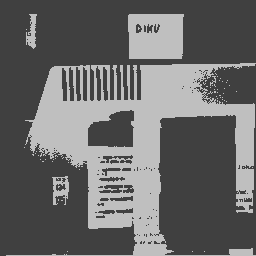
\includegraphics[width=0.3\textwidth]{images/r02}}
\subfloat[]{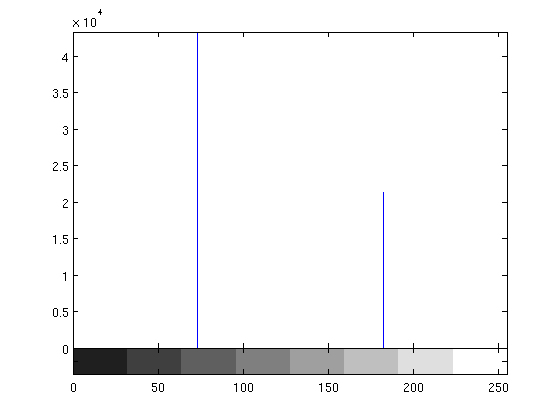
\includegraphics[width=0.45\textwidth]{images/r02h}}
\caption{Reduced to 2 gray colors, image and histogram}
\label{fig:reduceGray2}
\end{figure}

\subsubsection*{Resolution change}
We now move on to changing the resolution of the picture. For convinience the images are kept in the original size, but the pixels are collapsed together. Alot of schemes can be chosen when reducing the resolution. A possibility would be to remove the number of pixel one would choose as factor and combine the rest into the new image. This would result in alot of information loss. Instead I have chosen to average over squares the size of the factor, and dealing with special cases if the image size is not a multiple of the input factor. The special cases to consider is if the factor is not multiple of the image size. This leaves some options to decide upon. I have chosen to take the $\mod$ between the image size and the factor to figure out the remainder of each axis, then if surpus divided by the resolution factor:
\[
\frac{overHang_{\{m|n\}}}{factor} < 0.5
\]
Then I expand either $m$ or $n$ to make it a multiple of the factor. This makes the image larger and fill the new pixel with values $0$ meaning it becomes black. To avoid this I copy the last column or row from the original picture, this makes it more realistic. And even better solution would be to center the original picture within the new frame and then copy the egdes outwards and dealing with the corners by making those the mean of the adjencent egdes. If it is larger then I choose to truncate the image to the nearest image size being and multiple of the factor.

\begin{figure}[!h]
\centering
\subfloat[]{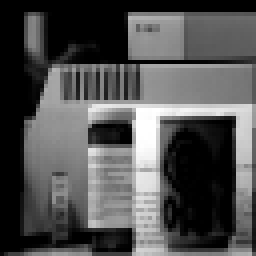
\includegraphics[width=0.3\textwidth]{images/rf04}}
\subfloat[]{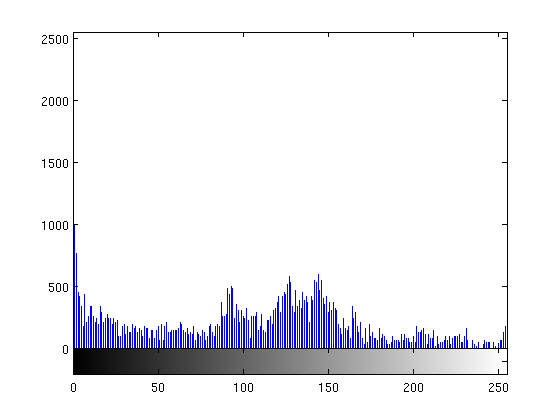
\includegraphics[width=0.45\textwidth]{images/rf04h}}
\caption{Resolution changed by factor 4, image and histogram}
\label{fig:resolutionFactor4}
\end{figure}

All of the texual information in the picture is loss by changing the resolution by a factor of 4 (see figure \ref{fig:resolutionFactor4}). The histogram are starting to clot together as a result of the squares being meaned. Most of the items in the image can still be seen. The pattern on the cup is somewhats distinguishable, although not very clear. Everything has gotten straight egdes.

\begin{figure}[!h]
\centering
\subfloat[]{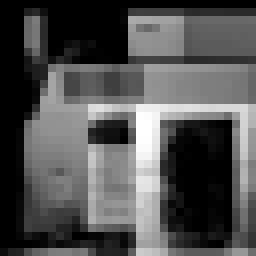
\includegraphics[width=0.35\textwidth]{images/rf08}}
\subfloat[]{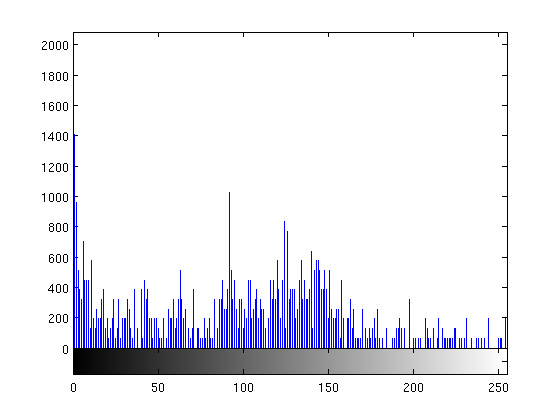
\includegraphics[width=0.45\textwidth]{images/rf08h}}
\caption{Resolution changed by factor 8, image and histogram}
\label{fig:resolutionFactor8}
\end{figure}

When the resolution factor is changed to 8 (see figure
\ref{fig:resolutionFactor8}) the measuring tape and cup is no longer
visible. The pattern on the cup now appears as a dark cloud is
pixels. The prescription is somewhats still distinguishable if you now
what your looking for, overwise its just two dark clouds with a
squared patch of white in between. The values in the histogram now
shows $8 \times 8$ squared being meaned therefore some of the values
now spike and gets a large count.

\begin{figure}[!h]
\centering
\subfloat[]{
\includegraphics[width=0.35\textwidth]{images/rf16}}
\subfloat[]{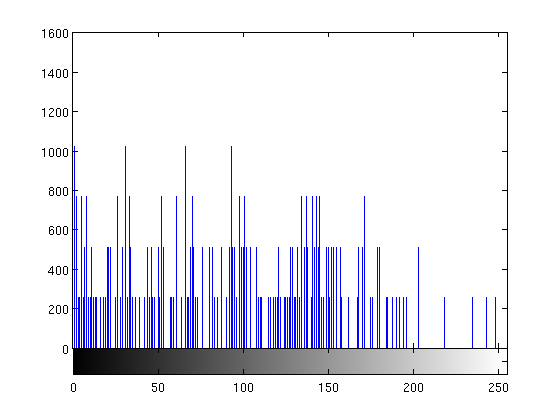
\includegraphics[width=0.45\textwidth]{images/rf16h}}
\caption{Resolution changed by factor 16, image and histogram}
\label{fig:resolutionFactor16}
\end{figure}

When considering figure \ref{fig:resolutionFactor16} with resolution factor 16, the image now only appears as large squares containing being the same color. It is no longer possible to identify any of the original objects. The histogram now shows that many of the colors now have the same count, this is a result of performing mean on the $16 \times 16$ squares of pixels.

%%%%%%%%%%%%%%%%%%%%%%%%%%%%%%%%%%%%%%%%%%%%%%%%%%%%%%%%%%%%%%%%%%%%
% Formal stuff

%\bibliographystyle{abbrvnat}
%\bibliography{bibliography}
%\addcontentsline{toc}{chapter}{Litteratur}

\end{document}

% vim: set tw=72 spell spelllang=en:
